\documentclass[10pt]{scrartcl} % use larger type; default would be 10pt

\usepackage[utf8]{inputenc} % set input encoding (not needed with XeLaTeX)
\usepackage[cm]{fullpage}
\usepackage{amsmath}
\usepackage{caption}
\usepackage{float}
\usepackage{graphicx} % support the \includegraphics command and options
% for osx:
% \usepackage[backend=biber]{biblatex} % use biber command to regenerate references
% for ubuntu:
\usepackage{biblatex}
\usepackage{subcaption}

\renewcommand{\bibfont}{\footnotesize}
%\pagenumbering{gobble}
\usepackage{hyperref}
\addbibresource{report.bib}

\title{Accurate Vision-Based Landing For Multicopter UAVs}
\subtitle{CS280: Project Report}
\author{Constantin Berzan, Nahush Bhanage, Sunil Shah}
\date{}

\begin{document}
\maketitle

\begin{abstract}
Current approaches for automated landing of unmanned aerial vehicles (UAVs) are
based on GPS localization, which we show is quite inaccurate. We aim to improve
on this by using vision to locate a predefined target, and land on top of it.
We describe our progress towards this goal, our approach to pose estimation and
control, and the challenges we encountered.
\end{abstract}

%%%%%%%%%%%%%%%%%%%%%%%%%%%%%%%%%%%%%%%%%%%%%%%%%%%%%%%%%%%%%%%%%%%%%%%%%%%%%%
\section{Introduction}

Multicopter UAVs, colloquially known as \textit{drones}, have become
increasingly popular in recent years. This is thanks, in part, to the
appearance of affordable prototyping tools (such as the Arduino platform and 3D
printers), affordable sensors (such as the accelerometers used in smartphones),
and open-source autopilot software (such as ArduCopter by 3D Robotics). Today,
a hobbyist can buy an off-the-shelf UAV for less than a thousand US dollars,
and get it to fly in only a few hours, using the provided autopilot software.

There is increasing interest in commercial applications of UAVs, such as
precision agriculture and package delivery. For these applications to become a
reality, the UAVs' operation has to be entirely autonomous, from takeoff to
landing. The only approach to autonomous landing for which software is publicly
available today is based on GPS. The UAV records its takeoff location, and then
navigates back to that location in order to land.

{\bf What is the accuracy of GPS-based landing?} To find out, we ran the
following experiment 10 times: We placed a marker on the ground, placed the UAV
on top of it, flew it an arbitrary distance away, and then landed it
automatically using ArduCopter's \textit{return-to-launch} mode. We measured
the straight-line distance from the marker to the location where the UAV
actually landed. We obtained a mean of 195.33 cm and a standard deviation of
110.73 cm. While this might be sufficient when landing in an uninhabited field,
it is certainly not sufficient for landing in an inhabited area (for package
delivery) or for landing on a charging station (for precision agriculture).

{\bf The goal of our project} was to improve the accuracy of automated landing
by equipping the UAV with a camera, and using computer-vision techniques to
guide the UAV towards landing on a predefined marker. We made significant
progress towards this goal, although we were not yet able to demonstrate fully
autonomous landing. In this document we survey some prior work, present our
approach to pose estimation and control, show some accuracy and performance
results, and discuss the challenges we encountered. (This work is part of an
ongoing project to build an automated charging station for UAVs. Our code is
available as open source at {\tt https://github.com/cberzan/drones-287}.)


%%%%%%%%%%%%%%%%%%%%%%%%%%%%%%%%%%%%%%%%%%%%%%%%%%%%%%%%%%%%%%%%%%%%%%%%%%%%%%
\section{Prior Work}

The automated landing problem has been investigated in the research literature
of the early 2000s. Here we briefly describe the approaches taken by some of
the most cited papers on this topic.

Sharp, Shakernia, and Sastry \cite{sharp_et_al_2001} designed an approach for
automatically landing an unmanned helicopter. Their landing target uses a
simple monochromatic design made up of several squares. Onboard the helicopter,
they use a pan-tilt-zoom camera and two embedded computers with Intel CPUs.
They discuss the details of their approach to pose estimation, but omit the
details of the helicopter controller. Using a real-time OS and optimized custom
code, they are able to get their vision system to operate at a rate of 30 Hz.

Our own approach in this project is modeled after that of Sharp et al. The main
differences are that (1) we use cheap off-the-shelf hardware, rather than
research-grade hardware; (2) our camera is stationary, it is not capable of
panning or tilting; and (3) we use off-the-shelf software components such as
ROS and OpenCV, rather than writing all of our code from scratch.

Saripalli, Montgomery, and Sukhatme \cite{saripalli_et_al_2002} designed
another approach for automatically landing an unmanned helicopter. They use a
monochromatic H-shaped landing target. Their onboard vision system detects this
landing target and outputs the helicopter's relative position with respect to
it. This is sent wirelessly to a behavior-based controller running on a ground
station, which then directs the helicopter to land on top of the target. They
are able to run their controller at 10 Hz this way. They are also using a
high-accuracy differential GPS system, and it is not clear how much their
differential GPS and vision systems contribute to a successful landing.

Garcia-Pardo, Sukhatme, and Montgomery \cite{garcia_pardo_et_al_2002} look at a
more general problem, where there is no pre-specified landing target, and their
helicopter has to search autonomously for a suitable clear area on which to
land.

%% Add comment re: further work since (i.e. landing on an unstable surface / moving boat).

%%%%%%%%%%%%%%%%%%%%%%%%%%%%%%%%%%%%%%%%%%%%%%%%%%%%%%%%%%%%%%%%%%%%%%%%%%%%%%
\section{Our Approach}

\subsection{Architecture}

Our goal was to use inexpensive, off-the-shelf hardware, rather than expensive
equipment that is only accessible to researchers. We used quadcopter components
made by 3D Robotics, together with their ArduCopter autopilot (frequently
referred to under its old name, ArduPilot Mega or APM) and associated GPS
module. This autopilot acts as a low-level controller that keeps the quadcopter
stable. It runs an unmodified version of the open-source autopilot code
provided by 3D Robotics.

We augmented the quadcopter with a BeagleBone Black embedded computer, which
uses a 1 GHz ARM CPU. (Since the ARM architecture is so different from x86,
the 1 GHz figure should not be compared to the frequency of modern-day Intel
CPUs, which are far more advanced, and expensive.) Using a powered USB hub, we
connected the autopilot to the BeagleBone. We also connected the webcam and a
Wi-Fi adapter this way.

% TODO:
% Estimated power consumption?
% Estimated cost of system?

On the BeagleBone, we installed a pre-built image of the Ubuntu 12.04
distribution, obtained from {\tt armhf.com}. We installed pre-built packages
for ROS groovy from the official ROS repositories. We compiled OpenCV 2.4.7 by
hand. We also installed roscopter, a third-party piece of software that reads
the state of the autopilot and makes it available via ROS, and also makes it
possible to send controls to the autopilot. Our software took the form of
several ROS nodes passing messages to one another. This is illustrated in
figure \ref{fig:rosnodes}.


\subsection{Corner Detection}

As a first step, we detect the corners of the landing platform in an image (see
Figure \ref{fig:corners}):

\begin{enumerate}
\setlength{\itemsep}{0pt}
\setlength{\parskip}{0pt}
\setlength{\parsep}{0pt}
\item{
    Denoise the image using a 3x3 median filter, and pass it through the Canny
    edge detector.}
\item{
    Identify contours and establish a tree-structured hierarchy among them.}
\item{
    Discard contours which are not four-sided convex polygons and which have an
    area less than an experimentally determined threshold value.  We look for
    four-sided polygons and not specifically for squares, since they will not
    appear as squares under perspective projection.}
\item{
    Using the contour hierarchy, determine a contour which contains 6 other
    contours. This contour represents the boundary of our landing platform.
    Store coordinates of the corners of these 6 inner contours.}
\item{
    Label the largest of the 6 polygons as 'A' and the farthest one from 'A' as
    'D'. Label polygons as 'B', 'C', 'E' and 'F' based on their orientation and
    distance relative to the vector formed by joining centers of 'A' and 'D'.}
\item{
    For each polygon, label corners in anti-clockwise order.}
\end{enumerate}


\subsection{Pose Estimation}

We define the origin of the world coordinate frame to be the center of the
landing platform, such that all points on the landing platform have a Z
coordinate of zero. The corner detector gives us image coordinates for the 24
corners. Thus, we have a set of 24 point correspondences between world
coordinates and image coordinates. Given this input, we want to compute the
quadcopter's pose, i.e. the position and orientation of the camera in the world
coordinate frame. To do this, we follow the approach of Sharp et al.
\cite{sharp_et_al_2001}, whose details we omit here for brevity. We use SVD to
approximately solve a linear system of 48 equations with 6 degrees of freedom.

The output from the pose estimator is a translation vector
$t = \begin{bmatrix} t_x & t_y & t_z \end{bmatrix}^\top$
and a 3x3 rotation matrix $R$. We compute the camera position in world
coordinates as $C = -R^\top t$, and the yaw angle as
$\alpha = \arctan(R_{21} / R_{11})$. (The roll and pitch angles can be computed
similarly, but we do not require them in the control algorithm.)

The approach above assumes a calibrated pinhole camera. For the pose estimates
to be meaningful, our camera had to be calibrated first. We calibrated our
camera using the {\tt camera\_calibration} tool provided in the OpenCV
tutorials, plus some manual tuning. We used the resulting calibration matrix to
convert the raw pixel coordinates into coordinates for a calibrated pinhole
camera model, which we then fed into the equations above.


\subsection{Control}

We defer real-time control of the UAV to the autopilot's \textit{loiter} mode.
This takes care of real-time stabilisation, and attempts to keep the UAV in the
same location using GPS. Our vision system then sends small corrections to
these controls, guiding the UAV towards the landing platform.

% TODO:
% It would be nice to describe how roscopter is limited, and we can only send
% PWM values for the channels, instead of controlling the roll, pitch, yaw,
% throttle directly. But we have no space.

Our controller takes the form of a state machine, illustrated in Figure
\ref{fig:statediagram}. The UAV starts out in the \textit{FLYING} state. When
landing is desired, it switches into the \textit{SEEK\_HOME} state. This uses
the autopilot's \textit{return-to-launch} mode to bring the UAV close to the
original takeoff location, using GPS. When the landing platform becomes
visible, the UAV switches into the \textit{LAND\_HIGH} state. Here we use our
vision-based pose estimates with a simple proportional controller to guide the
UAV towards the landing platform. (The error terms in our controller are given
as x, y, z, and yaw deviations. The controller descends at a fixed rate, using
the z deviation only as an estimate of the altitude.) When the UAV reaches a
predefined altitude (where pose estimates are no longer possible, due to
limited field of view), our controller enters the \textit{LAND\_LOW} state, and
descends slowly by dead reckoning. When the barometric pressure sensor indicates
that the UAV has reached the ground, the controller switches into the
\textit{POWER\_OFF} state.


%%%%%%%%%%%%%%%%%%%%%%%%%%%%%%%%%%%%%%%%%%%%%%%%%%%%%%%%%%%%%%%%%%%%%%%%%%%%%%
\section{Results}

\subsection{Pose Estimation Accuracy}
\label{sec:accuracy}

We tested the accuracy of our pose estimator in the lab, by holding the camera
above the landing pad, and comparing the true measured height to the height
reported by the pose estimator. We also measured the standard deviation in our
pose estimate, by taking multiple measurements of the same scene. We compared
the standard deviation on x and y to the lower bound given by the dimensions on
the ground plane that correspond to one pixel in a 640x480 image at a given
height. Table \ref{tab:pose-accu} shows these results. There is a small (1.4\%
relative) systematic overestimation of the true height. This can be corrected
by doing more precise calibration. The height estimate is very stable at these
heights (small standard deviation). The x and y estimates are also fairly
accurate, although the error in these estimates is an order of magnitude
greater than the lower bound. This is consistent with the fact that there is
some noise in the corner detection, and the pose estimator finds an approximate
solution. In summary, this experiment suggests that our pose estimates should
be good enough to reliably land our quadcopter. If individual measurements are
too noisy, it is possible to get better pose estimates using a Kalman filter,
although that requires having a model of the dynamics and controls of the
system.

\begin{table}[h!]
    \centering
    \begin{tabular}{c|cc|cc|cc|c}
        true height & z mean    & z std     & x bound   & x std     & y bound   & y std     & yaw std \\
        \hline
         88 cm      & 89.3 cm   & 0.05 cm   & 0.19 cm   & 0.43 cm   & 0.14 cm   & 0.39 cm   & 0.12 $^{\circ}$ \\
        120 cm      & 121.1 cm  & 0.08 cm   & 0.26 cm   & 1.16 cm   & 0.19 cm   & 1.06 cm   & 0.12 $^{\circ}$ \\
        170 cm      & 172.0 cm  & 0.18 cm   & 0.37 cm   & 2.74 cm   & 0.27 cm   & 2.17 cm   & 0.07 $^{\circ}$ \\
        226 cm      & 229.0 cm  & 0.54 cm   & 0.49 cm   & 6.51 cm   & 0.36 cm   & 6.05 cm   & 0.34 $^{\circ}$ \\
    \end{tabular}
    \caption{
        Accuracy of our pose estimates. ``x bound'' and ``y bound'' are lower
        bounds for the error on x and y, given by the limited image resolution.
    }
    \label{tab:pose-accu}
\end{table}

\subsection{Performance on the Embedded Computer}

When running on a modern-day laptop, our system easily achieves 30 frames per
second (FPS), the upper bound dictated by the camera we are using.
Unfortunately, performance is much slower on the embedded BeagleBone computer.
Just capturing frames from the camera puts significant strain on the system,
and we are only able to get 11.2 FPS, even if we perform no processing on the
frames. Adding the pose estimation code reduces performance to 3.0 FPS, and
running roscopter at the same time further reduces performance to 1.6 FPS.

These disappointing performance numbers point to a fundamental tradeoff when
developing a system such as ours: One could use off-the-shelf software packages
like ROS and OpenCV, which reduce development time, or one could talk directly
to the hardware and write all the code from scratch, which guarantees top
performance. Sharp et al \cite{sharp_et_al_2001} achieved 30 FPS with their
custom-code approach. Our experience suggests that even a decade later, it is
impractical to achieve good performance if we rely too much on third-party
libraries.


%%%%%%%%%%%%%%%%%%%%%%%%%%%%%%%%%%%%%%%%%%%%%%%%%%%%%%%%%%%%%%%%%%%%%%%%%%%%%%
\section{Challenges}

This section describes the challenges we have encountered, and should be
especially helpful to someone trying to replicate or extend our project. We
discuss some potential solutions in the next section.

\subsection{Platform Integration}

We spent an unexpectedly large amount of time addressing integration issues.
The first two USB hubs we tried did not work reliably with the BeagleBone,
failing to be recognized if they were plugged in at boot time. The first Wi-Fi
adapter we tried did not support ad-hoc networking, despite the manufacturer's
claims to the contrary. In addition, the hastily written documentation for
roscopter mentioned the {\tt --rate} parameter instead of {\tt --baud-rate},
leading to baffling failures to communicate with the APM, until we dug into
this third-party code and found the problem.\footnote{We have released a
corrected and somewhat cleaned-up version of roscopter at {\tt
https://github.com/cberzan/roscopter}.}

Another issue was that our webcam tried to automatically adjust exposure and
focus, which led to unfocused or over-exposed images in the field. After
extensive trial-and-error, we figured out how to tell the hardware to keep the
exposure and focus at fixed values, but this required that we run an experiment
to determine these values each time we went to fly our quadcopter.

Our main lesson from this experience is that we should not underestimate the
amount of time it takes to assemble and validate a new hardware platform for
running experiments. It is doubtlessly much quicker to get started with a
platform that others have already validated, or to use a software simulation.

\subsection{Field of View and Sensor Limitations}

We measured our camera's field of view to $69^\circ$ on the long side and
$42^\circ$ on the short side. This means that at a height of one meter, we see
an area of 1.37 m by 0.77 m on the ground. Our landing platform is about 0.76 m
by 0.76 m. This means that at a height of one meter, the UAV has to be exactly
above the landing pad in order to see all of it. (We get pose estimates only if
we see all the corners of the landing pad.) Since the UAV is rarely exactly
above the landing platform, the limited field of view is also a problem at
heights above one meter.

We thought that we would guide the UAV to a height of one meter using vision,
and then land using dead reckoning. The latter turned out to be difficult for
two reasons. First, airflow effects near the ground made the motion of the UAV
unpredictable. Second, there was a lot of drift in the barometer data, so we
were unable to get reliable height estimates below one meter, and thus our
controller could not tell when to \textit{POWER\_OFF}.

When the landing platform was in sight, we still sometimes failed to detect
corners because of blurry images. These are caused by camera shake, and are
especially problematic in lower-light conditions such as a cloudy day. Figure
\ref{fig:badimage} shows an example image.

\subsection{Weather}

Two aspects of weather led to difficulties. First, the cold temperature
affected the batteries, reducing flight time to a meager 5 minutes.  Second,
our controller struggled with gusts of wind. We relied on the autopilot's
GPS-based \textit{loiter} mode to keep the UAV in place while the vision system
sent small adjustments to the controls. In windy conditions, there was
significant drift in \textit{loiter} mode.


%%%%%%%%%%%%%%%%%%%%%%%%%%%%%%%%%%%%%%%%%%%%%%%%%%%%%%%%%%%%%%%%%%%%%%%%%%%%%%
\section{Future Work and Conclusion}

To improve the field of view at low heights, we are considering a modified
design for the landing platform. It is also possible to use a fish-eye lens to
get a wider field of view. We are also working on a full PID controller, which
would provide more aggressive control in windy conditions. It is also critical
to optimize our code and hardware stack so that we can get pose estimates at a
higher frequency.

Although we were unable to demonstrate an accurate landing using vision, we
made significant progress towards this goal. We demonstrated accurate pose
estimation using a known landing target, and made our code available online.
Although a proof-of-concept demonstration is within reach, our system requires
significant testing before it can be used as an off-the-shelf component.


%%%%%%%%%%%%%%%%%%%%%%%%%%%%%%%%%%%%%%%%%%%%%%%%%%%%%%%%%%%%%%%%%%%%%%%%%%%%%%
\printbibliography

%%%%%%%%%%%%%%%%%%%%%%%%%%%%%%%%%%%%%%%%%%%%%%%%%%%%%%%%%%%%%%%%%%%%%%%%%%%%%%

% Figures moved here because we need to put them together to save space.

\clearpage

\begin{figure}[h!]
\centering
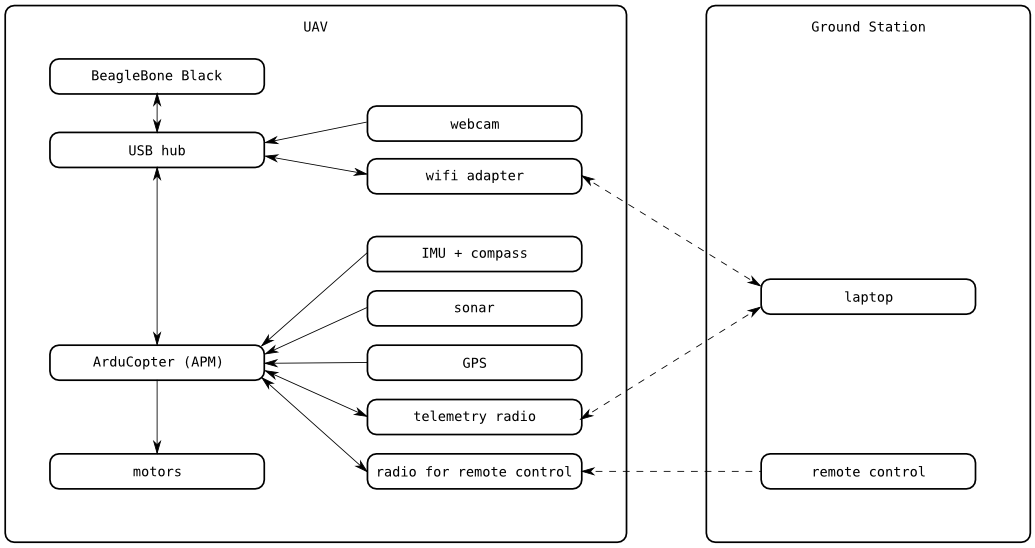
\includegraphics[width=0.9\textwidth]{images/architecture.png}
\caption{
    Architecture of our automated landing system. We use inexpensive
    off-the-shelf hardware. The laptop and remote control are for
    monitoring and emergency takeover by a human pilot. All the
    computation is performed onboard the UAV.
}
\label{fig:hardware-arch}
\end{figure}

\begin{figure}[h!]
\centering
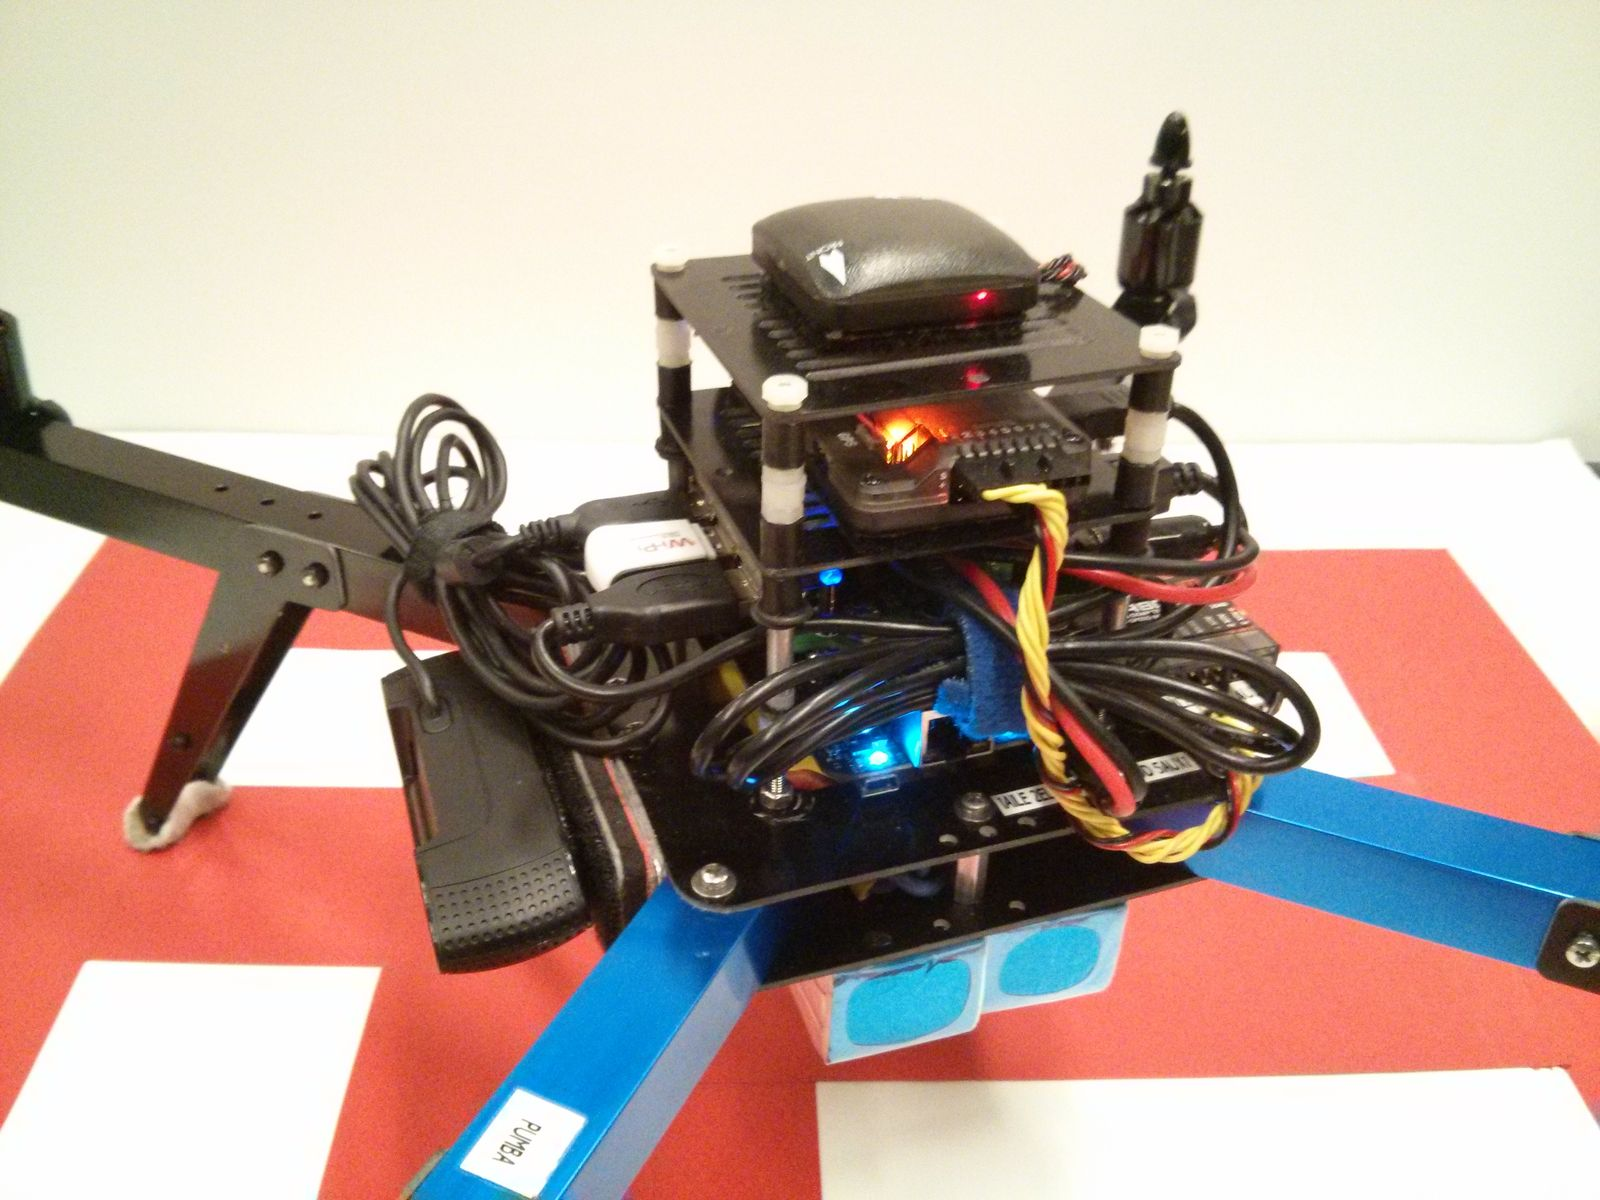
\includegraphics[width=0.85\textwidth]{images/hardware.jpg}
\caption{
    Our hardware stack fully assembled. From bottom to top: batteries,
    BeagleBone embedded computer, USB hub with Wi-Fi adapter, 3D
    Robotics autopilot with embedded sensors, GPS module. The
    webcam is on the left, and the radio for the remote control is on
    the right. Total weight excluding batteries is 1.35 kg.
}
\label{fig:hardware-photo}
\end{figure}

\begin{figure*}[h]
    \centering
    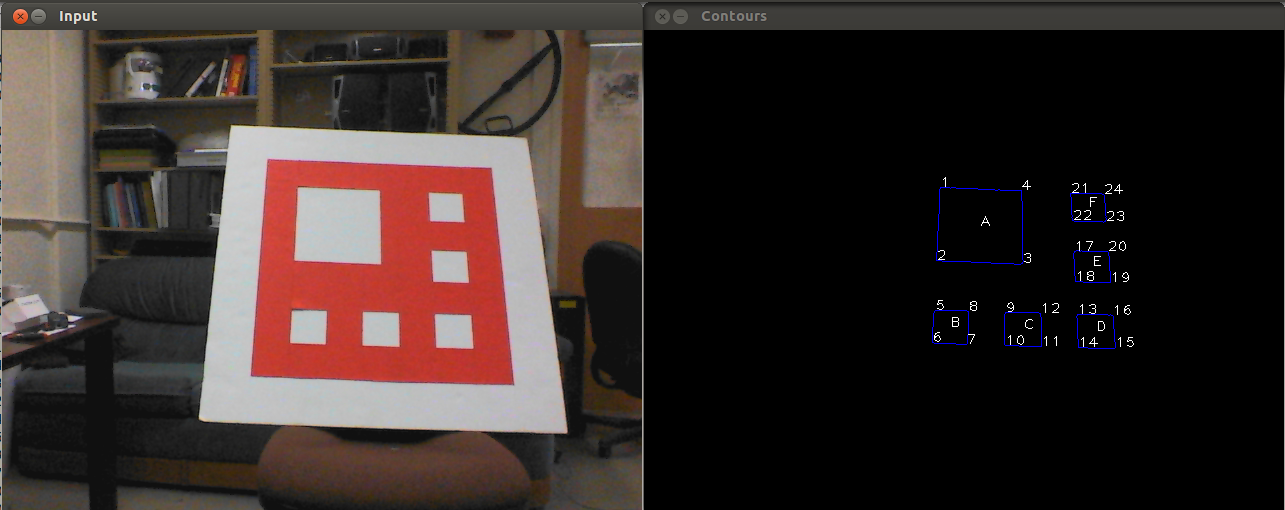
\includegraphics[width=\textwidth]{images/corners.png}
    \caption{
        Left: Design of our landing platform.
        Right: Output of the corner detector (24 points, in order).
    }
    \label{fig:corners}
\end{figure*}

\begin{figure}
    \begin{minipage}{0.5\textwidth}
        \centering
        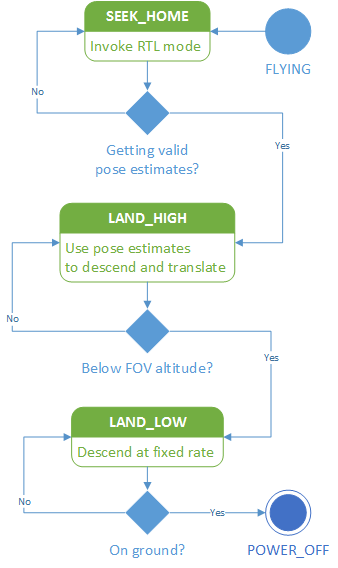
\includegraphics[width=0.9\linewidth]{images/statediagram.png}
        \caption{State diagram of our landing controller.}
        \label{fig:statediagram}
    \end{minipage}% this comment necessary, otherwise extra newline treated as space
    \begin{minipage}{0.5\textwidth}
        \centering
        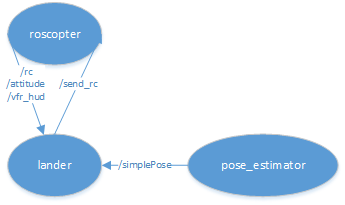
\includegraphics[width=0.9\linewidth]{images/rosnodes.png}
        \caption{ROS nodes and topics for exchanging messages.}
        \label{fig:rosnodes}
        \vspace{2cm}
        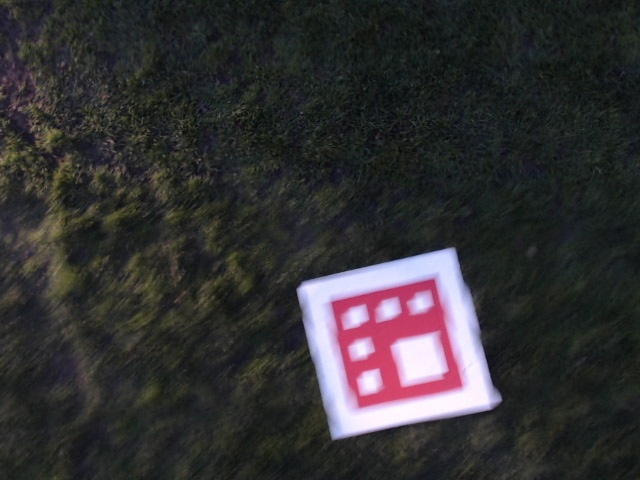
\includegraphics[width=0.9\linewidth]{images/badimage.jpg}
        \caption{An image where pose estimation fails.}
        \label{fig:badimage}
    \end{minipage}
\end{figure}

\end{document}
